% !TEX TS-program = pdflatexmk

\documentclass[modern]{aastex61}
\usepackage[utf8]{inputenc}
\usepackage{hyperref}
\usepackage{natbib}
\usepackage{graphicx}
\usepackage{xspace}
\usepackage{amsmath}
\usepackage{amssymb}
\usepackage{mathrsfs}

\include{macros}
% Journals


% Astronomical abbreviations (thanks to Dan Huber)
\newcommand{\numax}{\mbox{$\nu_{\rm max}$}\xspace}
\newcommand{\Dnu}{\mbox{$\Delta \nu$}\xspace}
\newcommand{\dnu}{\mbox{$\delta \nu$}\xspace}
\newcommand{\muHz}{\mbox{$\mu$Hz}\xspace}
\newcommand{\teff}{\mbox{$T_{\rm eff}$}\xspace}
\newcommand{\logg}{\mbox{$\log g$}\xspace}
\newcommand{\feh}{\mbox{$\rm{[Fe/H]}$}\xspace}
\newcommand{\msun}{\mbox{$\mathrm{M}_{\odot}$}\xspace}
\newcommand{\lsun}{\mbox{$\mathrm{L}_{\odot}$}\xspace}
\newcommand{\mearth}{\mbox{$\mathrm{M}_{\oplus}$}\xspace}
\newcommand{\rsun}{\mbox{$\mathrm{R}_{\odot}$}\xspace}
\newcommand{\kepler}{\emph{Kepler}\xspace}
\newcommand{\hipparcos}{\emph{Hipparcos}\xspace}
\newcommand{\gaia}{\emph{Gaia}\xspace}
% \newcommand{\ktwo}{\textit{K2}\xspace}
\newcommand{\ktwo}{\emph{K2}\xspace}
\newcommand{\ksc}{{\sc k2sc}\xspace}
\newcommand{\ksf}{{\sc k2sff}\xspace}
\newcommand{\kms}{\,km\,s$^{-1}$} % kilometres per second
\newcommand{\bibtex}{\textsc{Bib}\!\TeX} % bibtex. Not quite the correct typesetting, but close enough

\newcommand{\guy}[1]{{\bf \color{blue} #1}}

\begin{document}

\title{Detection of Oscillations in Aldebaran with Ground-Based Observations}

\author[0000-0003-1540-8562]{Will M. Farr} 

\affiliation{Birmingham Institute for Gravitational Wave Astronomy,
  University of Birmingham, Birmingham, B15 2TT, United Kingdom}

\affiliation{School of Physics and Astronomy, University of
  Birmingham, Birmingham, B15 2TT, United Kingdom}

\author[0000-0002-4290-7351]{Guy R. Davies}

\affiliation{School of Physics and Astronomy, University of
  Birmingham, Birmingham, B15 2TT, United Kingdom}
\affiliation{Stellar Astrophysics Centre, Department of Physics 
and Astronomy, Aarhus University, Ny Munkegade 120, DK-8000 Aarhus C, Denmark}

\author[0000-0003-2595-9114]{Benjamin J. S. Pope}
\affiliation{Sydney Institute for Astronomy, School of Physics, University of Sydney, Sydney NSW 2006, Australia} 
\affiliation{Center for Cosmology and Particle Physics, Department of Physics, New York University, 4 Washington Place, New York, NY 10003, USA}
\affiliation{NASA Sagan Fellow}

\author{Thomas North}
\affiliation{School of Physics and Astronomy, University of Birmingham, Birmingham, B15 2TT, United Kingdom}
\affiliation{Stellar Astrophysics Centre, Department of Physics 
and Astronomy, Aarhus University, Ny Munkegade 120, DK-8000 Aarhus C, Denmark}

\author[0000-0002-6980-3392]{Timothy R. White}
\affiliation{Stellar Astrophysics Centre, Department of Physics 
and Astronomy, Aarhus University, Ny Munkegade 120, DK-8000 Aarhus C, Denmark}

\author{James Barrett}
\affiliation{Birmingham Institute for Gravitational Wave Astronomy,
  University of Birmingham, Birmingham, B15 2TT, United Kingdom}

\affiliation{School of Physics and Astronomy, University of
  Birmingham, Birmingham, B15 2TT, United Kingdom}

\author{Andrea Miglio}

\affiliation{School of Physics and Astronomy, University of
  Birmingham, Birmingham, B15 2TT, United Kingdom}
\affiliation{Stellar Astrophysics Centre, Department of Physics 
and Astronomy, Aarhus University, Ny Munkegade 120, DK-8000 Aarhus C, Denmark}

\author{Mikkel N. Lund}

\affiliation{Stellar Astrophysics Centre, Department of Physics 
and Astronomy, Aarhus University, Ny Munkegade 120, DK-8000 Aarhus C, Denmark}
\affiliation{School of Physics and Astronomy, University of
  Birmingham, Birmingham, B15 2TT, United Kingdom}


\email{w.farr@bham.ac.uk, G.R.Davies@bham.ac.uk, b.pope@sydney.edu.au, txn016@student.bham.ac.uk, jimbarrett27@gmail.com}

\begin{abstract}
The nearby red giant Aldebaran is suspected to host a gas giant planetary companion from decades of ground-based spectroscopic measurements of its Doppler shift. Using Gaussian Process-based Continuous Auto-Regressive Moving Average (CARMA) models, we confirm this suspected planet and show that this historic data also contains evidence of acoustic oscillations in the star itself, and verify this result with further dedicated ground-based spectroscopy and space-based photometry with the \kepler Space Telescope. From the frequency of these oscillations we determine the mass of Aldebaran to be $1.16 \pm 0.07$~\msun, and note that this implies its planet will have been subject to insolation comparable to the Earth for some of the star's main sequence lifetime. Our approach to sparse, irregularly sampled time series astronomical data has the potential to unlock similar measurements for hundreds of stars in archival data, and permits more flexible observing schedules in future. 
\end{abstract}

\section{Introduction}

Aldebaran, or $\alpha$~Tauri, is a well-known first-magnitude naked-eye red giant star, and has long been the subject of astronomical investigations. It was one of the first stars around which an extrasolar planet candidate was identified, by looking for Doppler shifts from the star's reflex motion around the common centre of mass with its companion \citep[the radial velocity or RV method;][]{struverv}. While the hot Jupiter 51~Peg~b \citep{51peg} was the first exoplanet to be recognized as such, before this, \citet{hatzes1993} had noted RV variations in Pollux \citep[$\beta$~Gem; subsequently confirmed as a planet:][]{betgemconf,betgemconf2}, Arcturus ($\alpha$~Boo, unconfirmed), and Aldebaran. After further investigation by \citet{Hatzes1998}, \citet{Hatzes2015} have now claimed a firm RV detection of a planetary-mass companion Aldebaran~b, with a period of $628.96 \pm 0.90$~d. 

In this paper, we present a re-analysis of these original RV data in which we not only confirm this signal, but detect acoustic oscillations in Aldebaran for the first time. We validate this method and its result with new independent RV observations with the SONG~Telescope, and photometry from the \ktwo Mission. By measuring the frequency of maximum power, \numax, of these \emph{p}-mode oscillations we asteroseismically determine the mass of Aldebaran to be $1.16 \pm 0.07$~\msun. This measured stellar mass allows us to calculate that any moons of this giant planet, although they are now likely to be very hot, may have had equilibrium temperatures comparable to that of the Earth when Aldebaran was on the main sequence, raising the possibility that they may have once been habitable.

Our new approach to asteroseismic data analysis, based on Continuous Auto-Regressive Moving Average (CARMA) models, can extract exoplanet signals together with measures of \numax from sparse and irregularly-sampled time series. An all-sky survey to find planetary companions and to precisely measure the masses of all nearby red giant stars is feasible with this new approach, and the required data either already exist in large exoplanet surveys, or are easy to obtain with ground-based telescopes.

\section{Asteroseismology of Red Giants}
Asteroseismology is a powerful tool for the charaterisation of red giant stars \citep[see][for a detailed review]{2013ARA&A..51..353C}.  Red giants are solar-type pulsators, they exhibit acoustic modes of oscillation that are both excited and damped by stellar convection.  In the frequency-power spectrum of either radial velocity of photometric observations, these modes of oscillation form an often intricate pattern of sharp peaks where the properties of the pattern can be mapped back to intrinsic stellar properties \citep[e.g.,][]{2016AN....337..774D}.  The easiest properties of the pattern to determine are the the frequency of maximum amplitude \numax and the so-called large separation \Dnu \citep{Kjeldsen95}.  The two observables are often referred to as the global average seismic parameters.

Stellar properties can be determined with the average seismic measures and effective temperature \teff.  A set of scaling relations exist that illustrate the constraint the global asteroseismic measures provide.  These scaling relations are understood to be approximate but never the less are commonly used for radius $R$, mass $M$, and surface gravity $g$:
\begin{eqnarray}
\left( \frac{R}{\mathrm{R_{\odot}}} \right) \simeq & \left( \frac{\nu_{\rm max}}{\nu_{\rm max, \odot}} \right) \, 
\left( \frac{\Delta \nu}{\Delta \nu_{\odot}} \right)^{-2} \, \left( \frac{T_{\rm eff}}{T_{\rm eff, \odot}} \right)^{0.5}, \\
\left( \frac{M}{\mathrm{M_{\odot}}} \right) \simeq & \left( \frac{\nu_{\rm max}}{\nu_{\rm max, \odot}} \right)^{3} \, 
\left( \frac{\Delta \nu}{\Delta \nu_{\odot}} \right)^{-4} \, \left( \frac{T_{\rm eff}}{T_{\rm eff, \odot}} \right)^{1.5}, \\
\left( \frac{g}{\mathrm{g_{\odot}}} \right) \simeq & \left( \frac{\nu_{\rm max}}{\nu_{\rm max, \odot}} \right) \, 
 \left( \frac{T_{\rm eff}}{T_{\rm eff, \odot}} \right)^{0.5}. \\
\end{eqnarray}
While the accuracy of these scaling relations is still a matter of ongoing work \citep[e.g.,][]{2017ApJ...844..102H}, stellar parameters can be estimated by comparing observables to parameter from models of stellar evolution. 

As can be seen from the scaling relations, asteroseismology can provide constraint on Mass, Radius, and surface gravity if \Dnu, \numax, and \teff can be measured.  In practise, for the higher luminosity red giants it is more straight forward to measure \numax than \Dnu.  Typical values for \numax might range from $0.1$ to $20 \rm\,\mu Hz$ for the luminous giants and $20$ to $50 \rm\,\mu Hz$ for red giants with luminosities similar to the red clump .  For the same sets of stars, \Dnu would take ranges from $0.02$ to $3 \rm\,\mu Hz$ and $3$ to $7 \rm\,\mu Hz$ depending on stellar mass and \teff (or metallicity which is considered more fundamental) \citep[e.g.,][]{2011A&A...525L...9M, 2013A&A...559A.137M}.  Hence, \numax requires less frequency resolution than \Dnu to establish a good measurement.

The ability to measure \numax and \Dnu, therefore, depends on the length and sampling rate of a data set.  For regularly spaced data, typically analysed using an estimate of the frequency-power spectrum, the Nyquist limit (half the sampling rate) and frequency resolution ($\sim 1/$~duration) are trivial to estimate. %For the historic data sets proposed here the typical length is \guy{blah} and typical sampling is \guy{blah}.  This in principle gives us access to measures of \numax for \guy{these types of stars} and \Dnu $\,$ \guy{for those types of stars}. 

\section{Time-Domain Models}

It is easy to observe Aldebaran and similarly-bright stars with ground-based spectroscopic instruments, typically only requiring short exposures that can be obtained even under adverse observing conditions. There is indeed a considerable archive of such observations already, as a legacy of radial velocity (RV) surveys conducted to find exoplanets. In most cases, however, these have not so far been useful for asteroseismology, because these RV data are sparsely and irregularly-sampled. Because we have to pause observations during the day, during poor weather conditions, or simply when targets of higher priority are being observed, we get time series of only a few points and which may have significant and uneven gaps. This introduces a window-function effect: the power spectrum as constructed for example by a Fourier transform, or a Lomb-Scargle Periodogram \citep{lomb,scargle}, is convolved with the Fourier transform of the window function, introducing strong sidelobes adjacent to real frequency peaks and causing crosstalk between adjacent frequency channels. This imposes significant limitations both on the signal-to-noise and frequency resolution of power spectra derived from linear methods such as the Lomb-Scargle periodogram, and in practice makes asteroseismology with these conventional approaches difficult or impossible from the ground for stars with oscillation periods ranging from $\sim 12$~h to $\sim$~a few days. 

If we apply nonlinear statistical inference methods this situation can be improved. \citet{brewer2009} show that a system of driven, damped harmonic oscillators such as we encounter in asteroseismology can be statistically modelled as a Gaussian Process, with a covariance kernel consisting of a sum of damped sinusoids. The hyperparameters of this process can be used to retrieve very accurate power spectral density distributions. Unfortunately, this is impractical for long time series, as the computational cost of evaluating this likelihood function scales as $\mathcal{O}(n^3)$. 

Reference \citet{Kelly2014}, compare to \citet{Foreman-Mackey2017}.

\section{Aldebaran}
Aldebaran is a red giant star with spectral type K5, one of the nearest such stars at a distance of only $19.96 \pm 0.38$~pc \citep{hipparcos}. Its position near the Ecliptic permits the determination of its angular diameter by lunar occultations and by interferometry \citep[$20.58 \pm 0.03$ mas;][]{richichi2005,1979ApJ...228L.111B,brown1979,panek1980}.

\subsection{SONG Observations}

\subsection{K2 Observations}

%In order to verify the results of the novel analysis presented above, we sought to obtain an independent detection of the oscillations of Aldebaran and compare the frequencies determined with the two methods. 
Aldebaran was observed with \ktwo \citep{howell14}, a two-wheeled revival of the \kepler Mission \citep{2010sci...327..977b}, under Guest Observer Program 130471 in Campaign~13, from 2017-03-08 to 2017-05-27. Aldebaran and similar high-luminosity K giants are well known to show photometric variability due to solar-like oscillations \citep{bedding2000}, and hence the continuous, high-precision K2 light curves allow an independent confirmation of our CARMA results.

As Aldebaran is extremely bright, it saturates the \kepler detector and it is therefore not possible to use standard photometry pipelines to extract a K2 lightcurve. We instead use halo photometry \citep[as originally implemented in][]{White2017}, whereby unsaturated pixels from the outer part of the large and complicated halo of scattered light around bright stars are used to reconstruct a light curve as a weighted linear combination of individual pixel-level time series, as described in Appendix~\ref{halo}. 

Figure \ref{k2_lightcurve} shows the light curve and power spectrum of the K2 observations of Aldebaran. We detect clear variability on a average timescale of $\sim$\,5\,days, consistent with the expected timescale for solar-like oscillations for a high-luminosity red giant. To measure global asteroseismic parameters we model the background variability in the Fourier domain using the methodology described in \citet{huber09}, yielding a frequency of maximum power of $\numax = 2.2 \pm 0.25\,\muHz$ and amplitude per radial mode of $1850 \pm 500$\,ppm. Due to the limited frequency resolution of the 70-day K2 timeseries we were unable to measure the large frequency separation \Dnu, which is expected to be on the order of $\approx$\,0.5\muHz.

Using the \textsc{k2ps} planet-search code \citep{k2ps,Pope2016} to examine this light curve, we search for transits across a wide range of periods, and find no evidence either of short-period planetary transits or an eclipsing stellar companion.

\begin{figure}
\centering
% 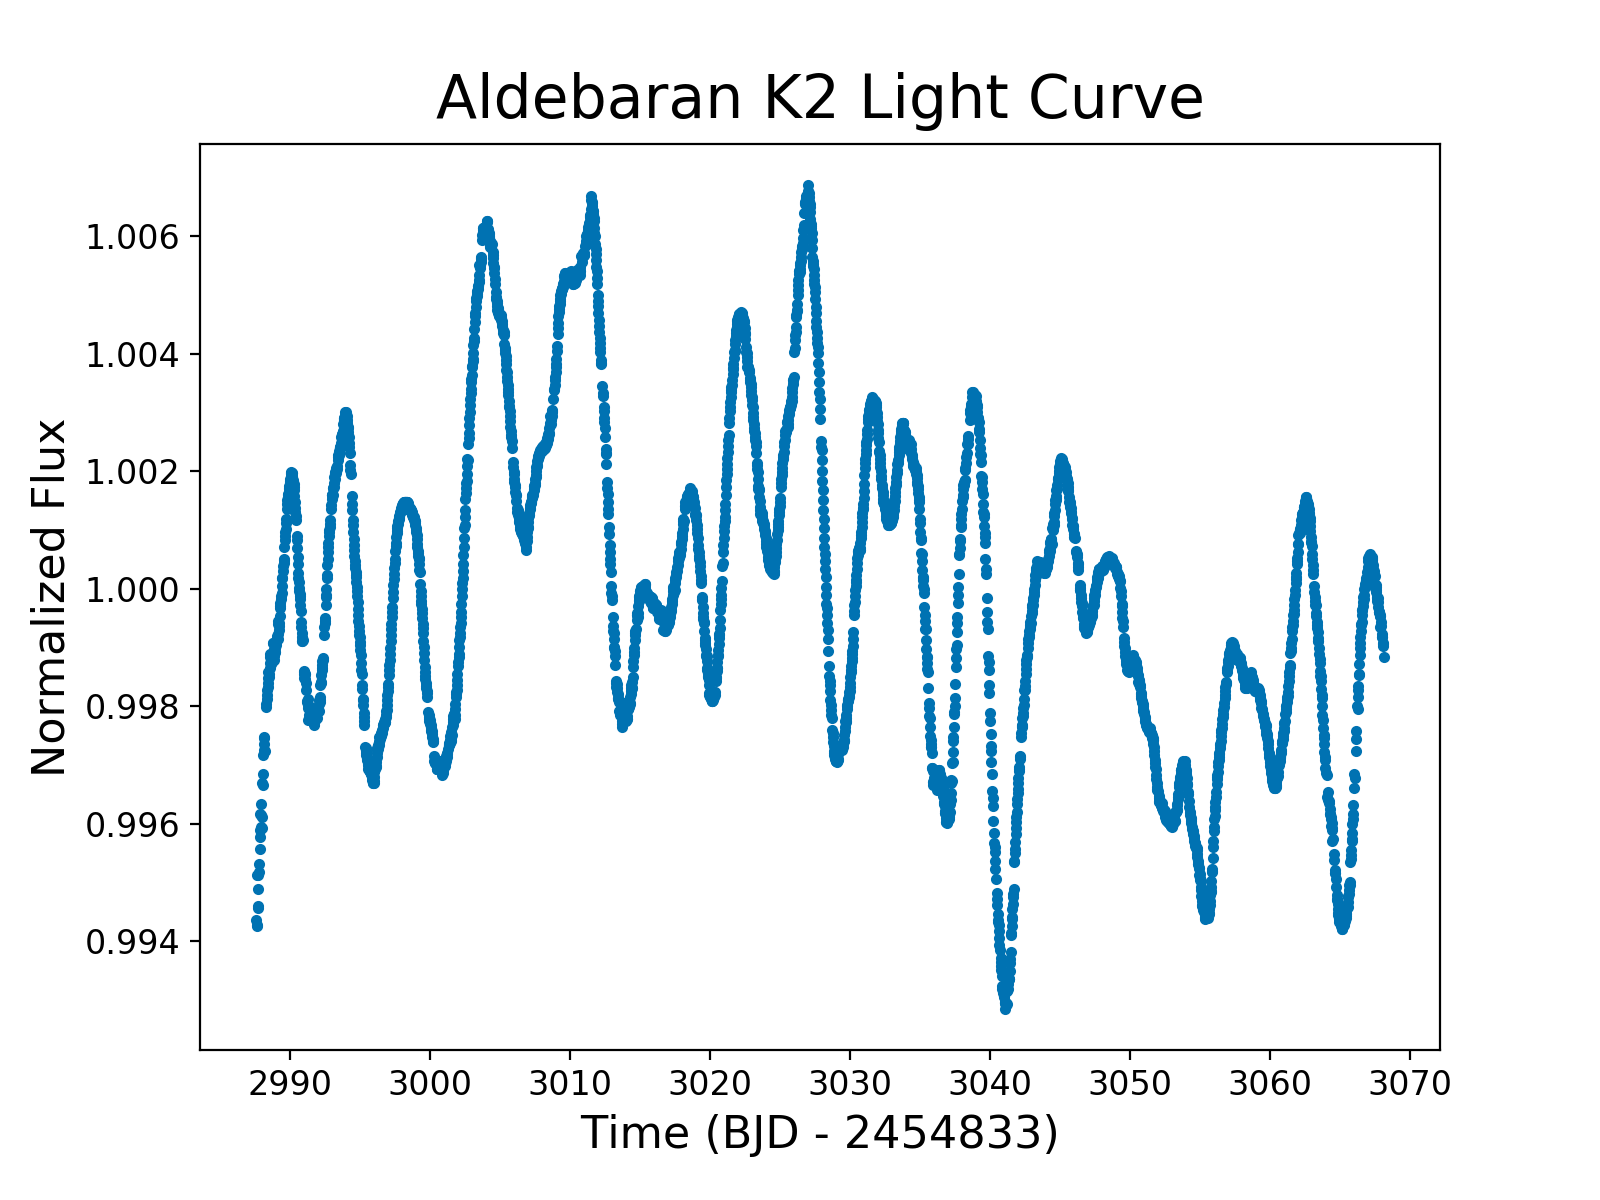
\includegraphics[width=0.75\textwidth]{Aldebaran_lc.png}
%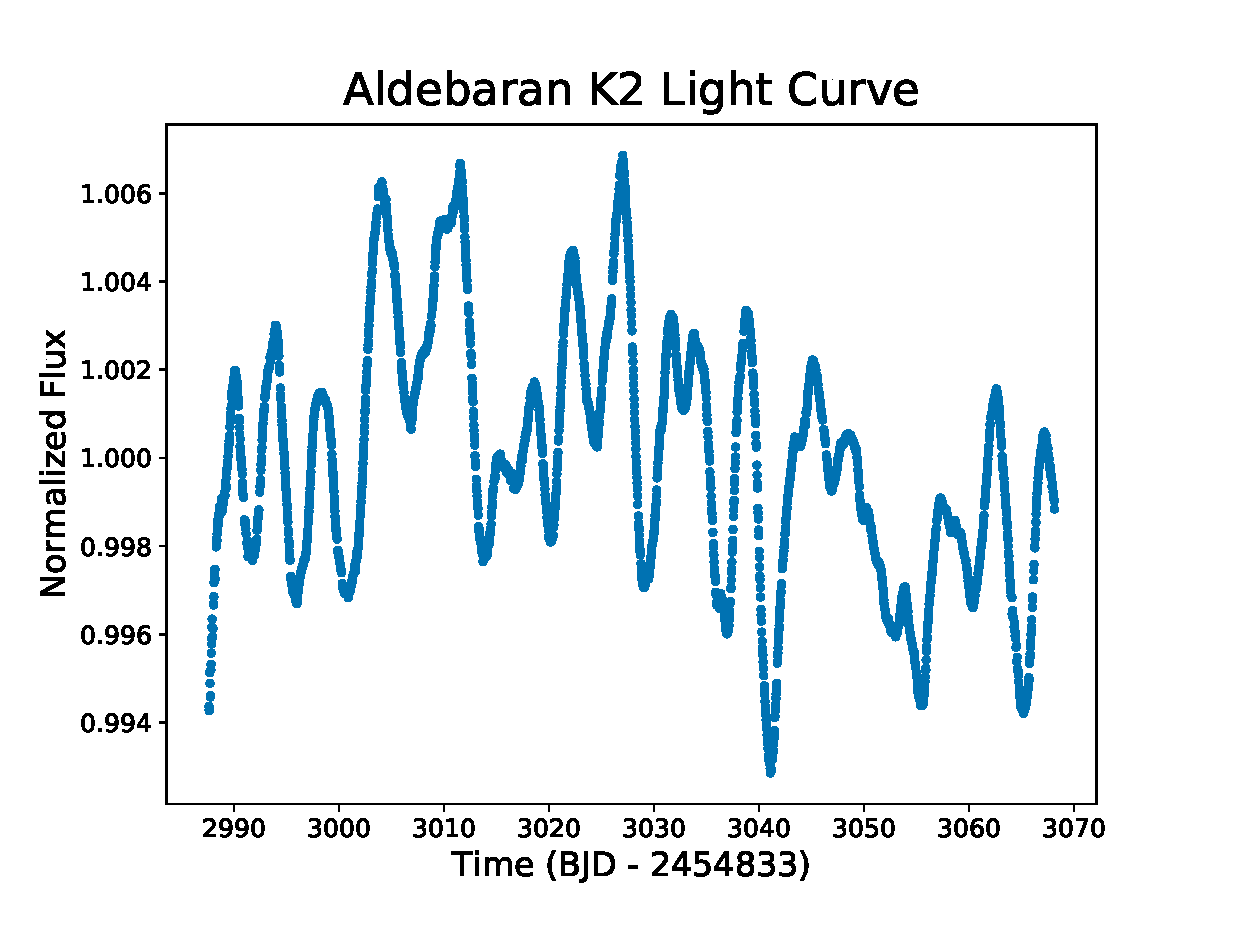
\includegraphics[width=0.75\textwidth]{aldebaran_lc.eps}
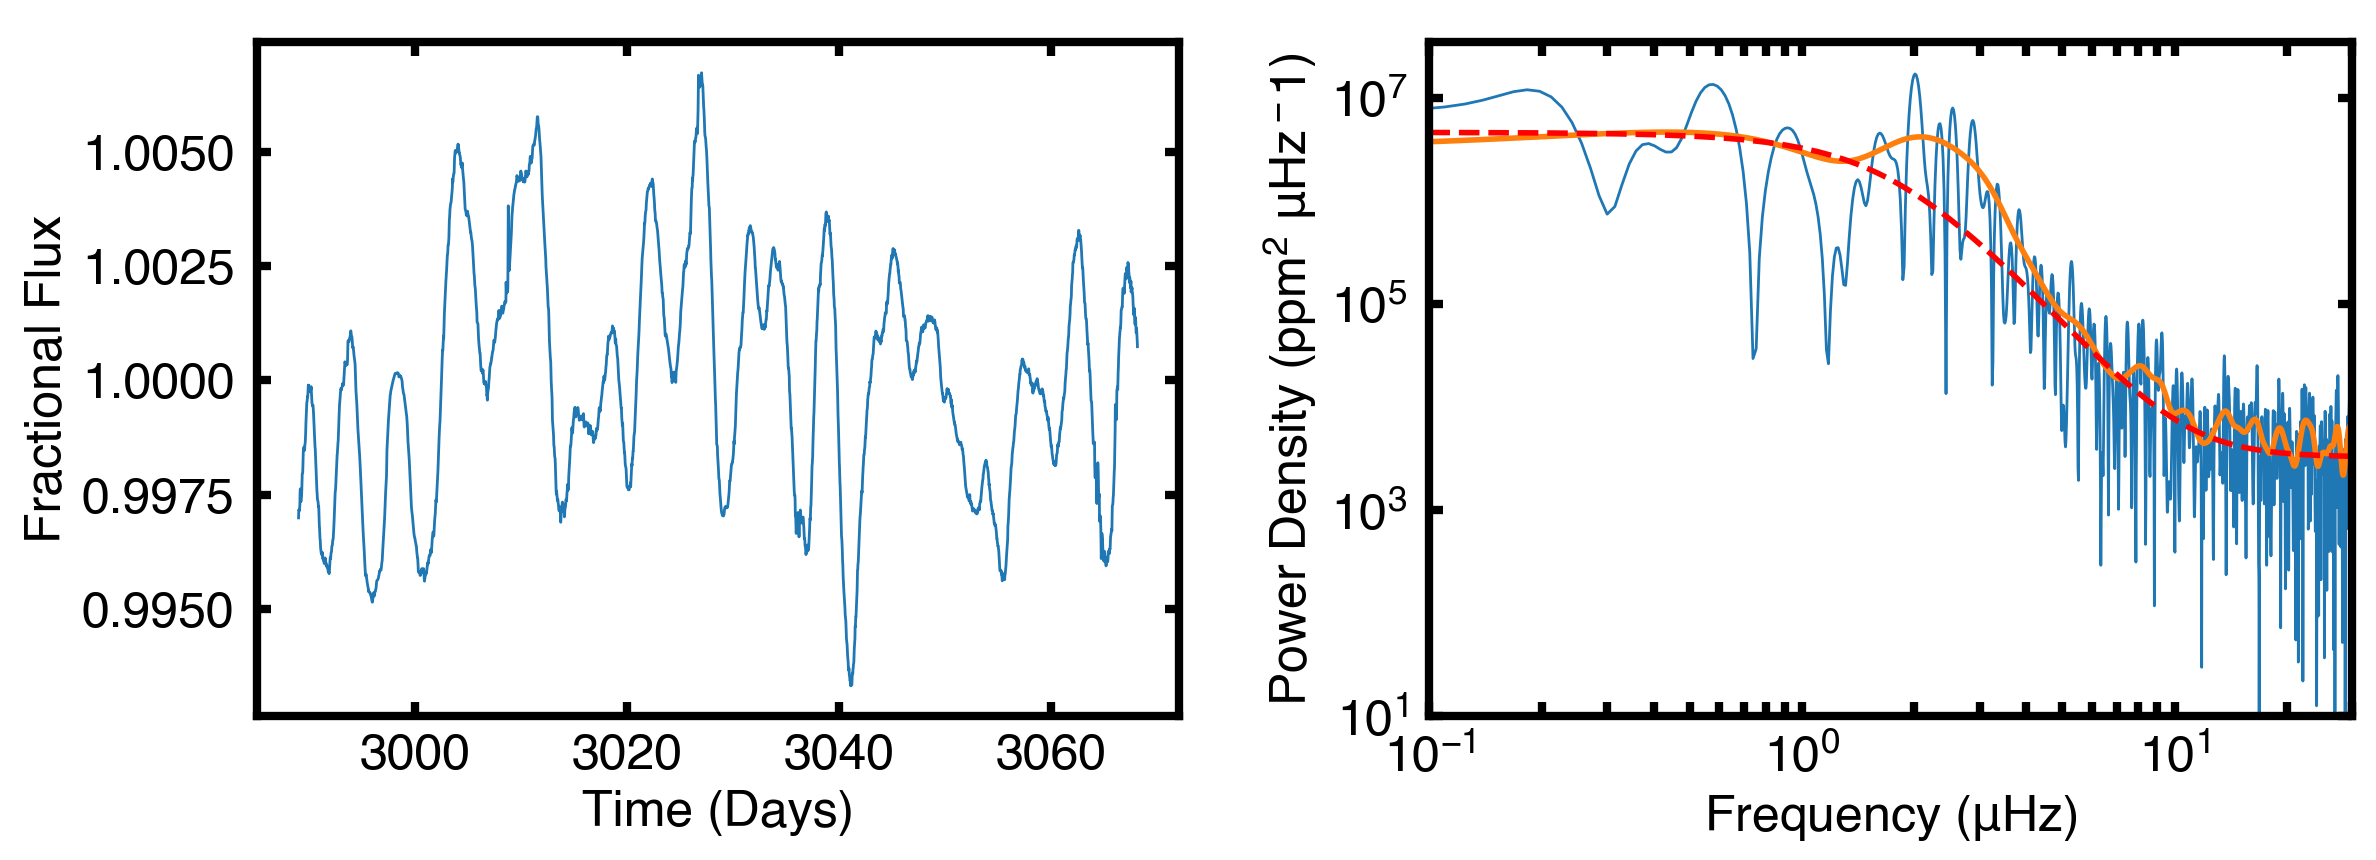
\includegraphics[width=\textwidth]{k2obs.png}
\caption{\ktwo lightcurve (left) and power spectrum (right) of Aldebaran. The red dashed line shows the background model, and the orange line is a heavily smoothed version of the power spectrum used to measure the frequency of maximum power. }
\label{k2_lightcurve}
\end{figure}

\subsection{Stellar Parameters}

We have determined the stellar properties of Aldebaran with the additional constraint of \numax determined from our analysis here.  The details of the stellar modelling are presented in detail in \ref{sec:mod}.  We have considered the impact of our additional \numax constraint and run our analysis for different sets of spectroscopic estimates.  For final values we adopt the \citet{2012Sheffield} spectroscopic solution as being `middle of the road' estimates.  For the analysis without constraint on \numax we find estimates of the stellar properties as $M = 1.27^{+0.24}_{-0.2} \, \mathrm{M_{\odot}}$ and age $4.86^{+3.56}_{-2.04} \, \rm Gyr$.  With the inclusion of \numax we find $M = 1.16^{+0.07}_{-0.07} \, \mathrm{M_{\odot}}$ and age $6.38^{+1.42}_{-1.12} \, \rm Gyr$.  It is clear that the addition of \numax provides substantially more precise estimates of mass and age.  % re sheffield - I have substituted the citation from the .bib but you said 'b'; afaik she only published one paper in 2012? - Ben

We note that with the determination of the stellar mass it is possible to infer the parameters Aldebaran had while it was on the main sequence. We conduct a Monte Carlo simulation, drawing masses randomly from a Gaussian distribution $M \sim \mathcal{N}(1.16,0.07)$ and metallicities $[\text{Fe}/\text{H}] \sim \mathcal{N}(-0.15,0.2)$ \citep{decin2003}  to predict the luminosity of the main-sequence progenitor, and the semi-major axis of the planet's orbit.  %Using the scaling relations of \citep{eker2015}, we find that Aldebaran would have had a luminosity $L_* = 2.0 \pm 0.37~\lsun$ on the main sequence.  
Using the Mesa Isochrones and Stellar Tracks \citep[MIST:][]{mist0,mist1} models via the \textsc{isochrones} package \citep{isochrones}, we compute the luminosity and radius evolution of the planet along the main sequence. $L$ evolves from $2.0 \pm 0.7$~\lsun at 0.5~Gyr to $3.5 \pm 2.3$~\lsun at 4.5~Gyr. 
We note that this implies that the planet at a semi-major axis of $1.507 \pm 0.03$~AU would have been subject to an insolation comparable to that of the Earth, evolving from 0.5~Gyr to 4.5~Gyr from $0.86 \pm 0.27$ to $1.55 \pm 1.0$ times that of the Earth today. Subject as well as this to the great uncertainties of the planet's orbital evolution and albedo, this planet and any of its moons may well have had temperate environments for some of their previous evolution, now long-since destroyed by their host star's evolution away from the main sequence. 

\section{Conclusions}

With CARMA models we have confirmed the previously-suspected planet around Aldebaran using archival data, and additionally detected acoustic oscillations that permit a $\sim 6\%$ mass determination. We have confirmed both of these results with new ground-based observations, and space-based photometry with \ktwo. 

From this pilot study with Aldebaran, have shown that with limited quantities of data of limited quality, we can nevertheless do precision asteroseismology from the ground and obtain very precise estimates of stellar parameters. Sufficient radial velocity data either already exist, or are trivial to obtain, in order to do this for essentially all bright giants; while for solar-like stars, these new methods allow significantly relaxed observing requirements. One rich archive is the series of observations with the Hamilton \'{E}chelle Spectrograph at Lick Observatory, studying 373 G~and K~giants \citep[e.g. ][]{frink2001,hekker2006,ortiz2016}. The method may also be useful in detecting rotational or other periodic variability in the LCES HIRES/Keck Precision Radial Velocity Exoplanet Survey \citep{butler2017} of 1,624 FGKM dwarfs, although the time sampling is by design too coarse to detect $p$-mode oscillations in these stars. Furthermore, CARMA models and related methods will enhance deep, all-sky, sparse photometric surveys such as \emph{Gaia} in space \citep{gaia}, or \emph{LSST} from the ground \citep{dmt,lsst,lsstbook}, from which many thousands of new asteroseismic determinations will be possible. An immediate future test of this will be from \hipparcos; while only~58 epochs of photometry are available for Aldebaran, a number and sampling insufficient for our purposes \textcolor{red}{check this is true}, stars at higher latitudes may often have 150--200 epochs and more even sampling \citep{hipparcos_phot}, and the~14 bright~K giants in \hipparcos noted by \citet{bedding2000} are an ideal first test case.

\acknowledgments

We thank the academy....

BP is grateful for funding from the Breakthrough Prize Foundation. This work was performed in part under contract with the Jet Propulsion Laboratory (JPL) funded by NASA through the Sagan Fellowship Program executed by the NASA Exoplanet Science Institute.
Funding for the Stellar Astrophysics Centre is provided by The Danish National Research Foundation. TRW acknowledges the support of the Villum Foundation (research grant 10118).
This research has made use of the SIMBAD database, operated at CDS, Strasbourg, France, and NASA's Astrophysics Data System. The \kepler data presented in this paper were obtained from the Mikulski Archive for Space Telescopes (MAST). STScI is operated by the Association of Universities for Research in Astronomy, Inc., under NASA contract NAS5-26555. Support for MAST for non-HST data is provided by the NASA Office of Space Science via grant NNX13AC07G and by other grants and contracts.  This work made use of the \textsc{IPython} package \citep{PER-GRA:2007}; SciPy \citep{scipy};  \textsc{matplotlib}, a \textsc{Python} library for publication quality graphics \citep{Hunter:2007}; \textsc{Astropy}, a community-developed core \textsc{Python} package for astronomy \citep{2013A&A...558A..33A}; and \textsc{NumPy} \citep{van2011numpy}. Some of the acknowledgements were compiled using the Astronomy Acknowledgement Generator.

\appendix

\section{Halo Photometry}
\label{halo}

The \kepler Space Telescope \citep{2010sci...327..977b}  
suffered a critical reaction wheel failure in May 2013, which made it impossible to maintain a stable pointing and therefore continue its nominal mission. It was revived as \ktwo \citep{howell14}, balanced by orienting perpendicular to the Sun. This requires that \ktwo observes fields in the Ecliptic in $\sim~80$~d Campaigns. 

The \kepler detector saturates for stars brighter than the $\sim~11^\text{th}$ magnitude. Nevertheless, the excess flux deposited in a saturated pixel spills conservatively up and down the pixel column, such that it is possible to sum this `bleed column' for bright stars and still obtain precise photometry, such as was done for the brightest star in the nominal \kepler mission, $\theta$~Cyg \citep[$V = 4.48$;][]{guzik2011,thetacygwhite,guzik2016}. There are two main reasons why this is not possible for all bright stars in general. First, because the downlink bandwidth from \kepler is very limited, it is often not desirable to download the large pixel stamps as are required for such bright stars; these must be even larger in \ktwo to account for the reduced image stability. Second, if the bleed column for a sufficiently bright star reaches the edge of the chip, flux spills over and is not conserved, imposing a hard brightness limit that depends on the distance to the detector edge. 
Collateral `smear' data, which are collected to help calibrate the photometric bias from stars sharing the same column as a target, can be used to reconstruct light curves for un-downloaded bright stars and thereby avoid bandwidth constraints \citep{k2smear}, but these data are still rendered unusable if the bleed column falls off the edge of the chip and contaminates the smear rows.

Bright stars have a wide, complicated, position-dependent point spread function (PSF) arising from diffraction and scattering from secondary and higher-order reflections inside the instrument, with the result that they may contaminate thousands of nearby pixels with significant flux. We can therefore use this `halo' of unsaturated pixels for photometry. The brightness of this halo varies in the same way as that of the primary star, and we therefore obtain data in a region of 20~pixel radius around the mean position of Aldebaran, and discard saturated pixels.
In this paper we proceed as in \citet{White2017}, in which the method was demonstrated on the seven bright Pleiades, with only minor changes.

The flux $f_i$ at each cadence $i$ is constructed as a weighted sum of pixel values $p_{ij}$:

\begin{equation}
	f_i = \sum_{j=1}^{M} w_j p_{ij}.
\end{equation}

\noindent We choose the weights $w_j$ such that they lie between 0~and~1, add to unity, and minimize the Total Variation (TV) of the weighted light curve. In the continuous case, $n$-th order TV is defined as the integral of the absolute value of the $n$-th derivative of a function; in the discrete case, replacing the derivative with finite differences, first-order TV becomes

\begin{equation}
\text{TV} = \dfrac{\sum_{i=1}^{N} |{f}_i - {f}_{i-1}|}{\sum_{j=1}^{N} {f}_j}
\end{equation}

\noindent and likewise second-order TV the equivalent expression in second-order finite differences. The efficacy of this method was recently confirmed by \citet{kallinger2017}, comparing BRITE-constellation observations of Atlas to \ktwo halo photometry and finding excellent agreement in frequency and amplitude of the reported oscillations.

In an improvement since \citet{White2017}, we use the \textsc{Theano} library \citep{theano} to calculate analytic derivatives for this objective function, which reduces the computational time for a single halo light curve on a commercial laptop from tens of minutes to tens of seconds. 

As a final step to reduce residual uncorrected systematics, we apply the \textsc{k2sc} \citep{k2sc} Gaussian Process-based systematics correction code to the initial halo light curve, but the effect of this in the present case for Aldebaran is minimal.
There is somewhat higher than usual residual noise at multiples of $4 c/d$ (the satellite thruster firing frequency), but this is nevertheless very small in comparison to the signal from Aldebaran, and may be ascribed to the large fraction of the pixel mask occupied by the bleed column from this extremely bright star.


\section{Stellar Modelling}\label{sec:mod}
\subsection{Stellar Models}\label{sec:stell_mod}
We used our determination of \numax and several combinations of the asteroseismic and spectroscopic parameters, along with luminosity, to estimate the fundamental stellar parameters, via fitting to stellar models. We used \textsc{MESA} models \citep{2011Paxton,2013Paxton} in conjunction with the Bayesian code \textsc{PARAM} \citep{2006dasilva, 2017Rod}.  A summary of our selected ``benchmark'' options is as follows; 
%%%%%%%%%%%%%%%%%%%%%%%%%%%%%%%%%%%%%%%%%%%%%%%%%%%%%%%%%%%%%%%%%%%%%%%%%%%%%%%%%%%%
\begin{itemize}%GUY THIS BIT COULD PROBABLY BE DROPPED AND REFERENCED OUT TO \citep{2017Rod}
\item Heavy element partitioning from \cite{1993Grevesse}.
\item OPAL equation of state \citep{2002Rogers} along with OPAL opacities \citep{1996Iglesias}, with complementary values at low temperatures from \cite{2005Ferguson}.
\item Nuclear reaction rates from NACRE \citep{1999Angulo}.
\item The atmosphere model is taken according to \cite{1966Kris}.
\item The mixing length theory was used to describe convection (a solar-calibrated parameter $\alpha_{\textrm{MLT}} =1.9657$ was adopted).
\item Convective overshooting on the main sequence is set to $\alpha_{\textrm{ov}}=0.2H_{p}$, with $H_{p}$ the pressure scale height at the border of the convective core. Overshooting was applied according to the \cite{1975Maeder} step function
scheme.
\item No rotational mixing or diffusion is included.
\end{itemize}
%%%%%%%%%%%%%%%%%%%%%%%%%%%%%%%%%%%%%%%%%%%%%%%%%%%%%%%%%%%%%%%%%%%%%%%%%%%%%%%%%%%%
Note that the precision on our estimate of \numax is orders of magnitude less that the point at which we would have needed to correct for the line-of-sight doppler shift \citep{2014MNRAS.445L..94D}.
\subsection{Additional modelling inputs}\label{sec:addmod}
In addition to the asteroseismic parameters, temperature and metallicity values are needed. There exist multiple literature values for Aldebaran. We chose to use a selection of sources as a separate modelling variation, to investigate what variation this would produce in final stellar properties. 

To ensure the values are self-consistent, when a literature value was chosen for temperature, we took the stellar metallicity from the same source i.e. matched pairs of temperature and metallicity. The final constraint is the stellar luminosity, which may be estimated as follows (e.g. see \citealt{pijpers2003}):
\begin{multline}
\log_{10} \frac{L}{L_{\odot}} = 4.0+
0.4 M_{{\textrm{bol}},\odot} -2.0 \log_{10} {\pi [{\textrm{mas}]}} \\-0.4(V-A_V + BC(V)).
\label{eqn:lum}
\end{multline}
The solar bolometric magnitude $M_{\textrm{bol},\odot}=4.73$ is taken from \cite{Torres2010}, from which we also take the polynomial expression for the bolometric correction $BC(V)$. Extinction $A_V$ was assumed to be zero.

The final constraint available for Aldebaran is the angular diameter of the star, measured by long baseline interferometry, combined with the parallax to produce a physical radius constraint of $R_{\textrm{int}}=44.2\pm0.9\textrm{R}_{\odot}$ \citep{richichi2005}.

% Example table
\begin{table*}
	\centering
	\caption{Spectroscopic from each literature source, along with calculated luminosity. All temperature uncertainties assumed to be 50K, 0.2 dex in $\log{g}$, and 0.1 dex in [FeH]. For the two \protect{\cite{2012Sheffield}} results, the reason for discrepancy between the two sets of metallicity results is not discussed.}
	\label{tab:spec}
	\begin{tabular}{lllll} % 5 columns, alignment for each
		\hline
		Spectrosocpy Source & $T_{\textrm{eff}}$ (K) & $\log{g}$ (dex) & [FeH] (dex) & Luminosity (L$_{\odot}$)\\
		\hline
		\cite{2012Sheffield}$_{a}$	&	3900	&	1.3	&	0.17	&	480\\
		\cite{2012Sheffield}$_{b}$	&	3900	&	1.3	&	0.05	&	480\\
		\cite{2011Prugniel}	&	3870 & 1.66 & -0.04 & 507\\
		\cite{2008Massarotti} & 3936 & 1 & -0.34 & 456\\
		\cite{2009Frasca} & 3850 & 0.55 & -0.1 & 526\\
		\hline
	\end{tabular}
\end{table*}

As Table \ref{tab:spec} shows, the spectroscopic parameters of Aldebaran are somewhat unclear, particularly $\log{g}$ and [FeH], which may have an impact on the recovered stellar properties when fitting to models. To explore what impact each parameter is having on the final stellar properties, multiple \textsc{PARAM} runs were performed, using different constraints. Two constraints potentially in tension were $\nu_{\textrm{max}}$ and $\log{g}$. $\nu_{\textrm{max}}$ has been shown to scale with $\log{g}$ \citep{Kjeldsen95, 2011A&A...530A.142B},
\begin{equation}
\frac{\nu_{\textrm{max}}}{\nu_{\textrm{max},\odot}}=\frac{\log{g}}{\log{g},\odot}\left(\frac{T_{\textrm{eff}}}{T_{\textrm{eff},\odot}}\right)^{-1/2}.
\label{eqn:numax}
\end{equation}

Using Eq \ref{eqn:numax} with the values in Table \ref{tab:spec} predicts $\nu_{\textrm{max}}$ in the range $0.5-6\mu$Hz. Reversing the equation to produce a predicted $\log{g}$ from the observed $\nu_{\textrm{max,obs}}=2.23\pm0.1\mu$Hz results in a predicted $\log{g}\sim1.2$ dex, using an assumed temperature of 3900K. The solar calibration values used here are $g_{\odot}=274$ms$^{-2}$, $\nu_{\textrm{max},\odot}=3150\mu$Hz and $T_{\textrm{eff},\odot}=5777$K. 

Table \ref{tab:res_mass} shows the results, for all modelling variations, both different inputs and different constraints. It shows that results with the addition of $\nu_{\textrm{max}}$ as a constraint exhibit in general smaller uncertainties, with or without the addition of $\log{g}$ as a constraint. 

Recovering the mass without the use of asteroseismic constraints produces considerable scatter on the results ($0.96-1.5\textrm{M}_{\odot}$), whilst the use of asteroseismology brings the mass estimates into closer agreement, with the exception of the very low metallicity solution of \cite{2008Massarotti}. Any systematic offset between asteroseismic masses and spectroscopic masses is sensitive to chosen reference mass, in agreement with \cite{2017North}.

Within the results of Table \ref{tab:res_mass}, the parallax of Aldebaran is contained within the angular diameter and the luminosity of the star. To avoid this, \textsc{PARAM} was also ran without luminosity constraint, the average absolute mass offset between the two sets of results was $<0.04\textrm{M}_{\odot}$ for the runs without $\nu_{\textrm{max}}$ constraint, and $<0.02\textrm{M}_{\odot}$ for the runs with $\nu_{\textrm{max}}$.

% Example table
\begin{table*}
	\centering
	
	\caption{Recovered stellar properties from \textsc{PARAM} using various constraints. Uncertainties quoted are the 68\% credible interval.}
	\label{tab:res_mass}
	\begin{tabular}{llll} % 5 columns, alignment for each
		\hline
		Spectroscopy Source & Mass ($\textrm{M}_{\odot}$) & Radius ($\textrm{R}_{\odot}$) & Age (Gyr)\\
		\hline
		\multicolumn{4}{c}{$\nu_{\textrm{max}}$, $\log{g}$, $T_{\textrm{eff}}$, $R_\textrm{int}$, L and [FeH].} \\
		\hline
		\cite{2012Sheffield}$_{a}$ &$1.17^{+0.07}_{-0.07}$&$43.9^{+0.9}_{-0.9}$&$6.47^{+1.39}_{-1.1}$\\
		\cite{2012Sheffield}$_{b}$&$1.17^{+0.07}_{-0.07}$&$43.8^{+0.8}_{-0.9}$&$6.35^{+1.4}_{-1.11}$\\
		\cite{2011Prugniel}&$1.17^{+0.07}_{-0.07}$&$43.9^{+0.9}_{-0.9}$&$6.23^{+1.4}_{-1.11}$\\
		\cite{2008Massarotti}&$1.13^{+0.07}_{-0.07}$&$43.5^{+0.9}_{-0.9}$&$5.95^{+1.37}_{-1.07}$\\
		\cite{2009Frasca}&$1.02^{+0.04}_{-0.04}$&$44.0^{+0.8}_{-0.8}$&$10.26^{+1.54}_{-1.45}$\\
		\hline
		\multicolumn{4}{c}{$\log{g}$, $T_{\textrm{eff}}$, $R_\textrm{int}$, L and [FeH].} \\
		\hline
\cite{2012Sheffield}$_{a}$&$1.43^{+0.26}_{-0.24}$&$43.8^{+0.9}_{-0.9}$&$3.53^{+2.72}_{-1.44}$\\
\cite{2012Sheffield}$_{b}$&$1.27^{+0.24}_{-0.2}$&$43.8^{+0.9}_{-0.9}$&$4.86^{+3.56}_{-2.04}$\\
\cite{2011Prugniel}&$1.25^{+0.22}_{-0.19}$&$43.8^{+0.9}_{-0.9}$&$5.02^{+3.47}_{-2.02}$\\
\cite{2008Massarotti}&$0.95^{+0.11}_{-0.05}$&$43.8^{+0.9}_{-0.9}$&$10.24^{+2.36}_{-3.08}$\\
\cite{2009Frasca}&$0.96^{+0.04}_{-0.04}$&$44.4^{+0.8}_{-0.8}$&$11.64^{+1.43}_{-1.8}$\\
		\hline
		\multicolumn{4}{c}{$\nu_{\textrm{max}}$, $T_{\textrm{eff}}$, $R_\textrm{int}$, L and [FeH].} \\
		\hline
\cite{2012Sheffield}$_{a}$&$1.17^{+0.07}_{-0.07}$&$43.9^{+0.9}_{-0.9}$&$6.51^{+1.41}_{-1.11}$\\
\cite{2012Sheffield}$_{b}$&$1.16^{+0.07}_{-0.07}$&$43.8^{+0.8}_{-0.9}$&$6.38^{+1.42}_{-1.12}$\\
\cite{2011Prugniel}&$1.16^{+0.07}_{-0.07}$&$43.9^{+0.9}_{-0.9}$&$6.43^{+1.48}_{-1.15}$\\
\cite{2008Massarotti}&$1.13^{+0.07}_{-0.07}$&$43.5^{+0.9}_{-0.9}$&$5.86^{+1.35}_{-1.05}$\\
\cite{2009Frasca}&$1.15^{+0.07}_{-0.07}$&$43.9^{+0.9}_{-0.8}$&$6.47^{+1.51}_{-1.17}$\\
		\hline
	\end{tabular}
	
\end{table*}





\bibliography{aldebaran}



\end{document}
